
\documentclass[a4paper,12pt]{article}
\usepackage{epstopdf}
\usepackage[utf8]{inputenc}
\usepackage[english]{babel}
\usepackage{enumerate}
\usepackage{mathtools}
\usepackage{hyperref}
\usepackage{float}
\usepackage[pdftex]{graphicx}   
\usepackage{multirow}
\usepackage{listings}
\lstset{
    language=matlab,
    basicstyle=\ttfamily
}

\title{TBMI26  \\
       Assignment 4}
\author{Martin Estgren \texttt{<mares480>}}
      
\begin{document}
 \pagenumbering{arabic}
    \maketitle % Generate.

\section{Q-learning}
  

  The \textbf{Q}uantity-function represents a function that calculate the quantity of a state-action combination. The Q values are initialized arbitrarily by the designer (many cases either 0,1 or random) before the world-sampling starts. Whenever a state $s$ and an action $a$ is selected in the sampling the corresponding value $Q(S,A)$ is modified (corrected) based on the new information.
  \begin{equation}
    Q(s_t,a_t) = Q(s_t,a_t) + \alpha * (R_{t+1} + \gamma * max_a(Q(s_{t+1},a))-Q(s_t,a_t))
  \end{equation}

which corresponds to learning the optimal policy for a given state and action over many iterations of the problem. $\alpha$ is the learning rate and $\gamma$ is the discount factor. 

$ max_a(Q(s_{t+1},a))$ can also be explained as the   the \textbf{V}alue-function represents the greatest expected reward for a given state. ignoring possible actions. 


A learning rule could be defined as $R(s_1,s_2,a) = -1$ meaning all states, apart from the terminal (since the reward always is 0 from the terminal state regardless of actions) will have a punishment if the agent traverses it. This will cause the agent to look for the shortest path to the terminal state. This can be compared to the experiment with the mouse and cold water where all states apart from the terminal state have a negative reward i.e. is cold water.

We initialize the expected value for moving to a node adjacent to the border as a negative infinity value. This should, if the q-learning algorithm is correctly implemented hinder the robot form ever walking to a point with a risk of exiting the world. 

\subsection{Static irritating blob}

\begin{figure}[H]
\centering
  \begin{minipage}[]{0.8\textwidth}
  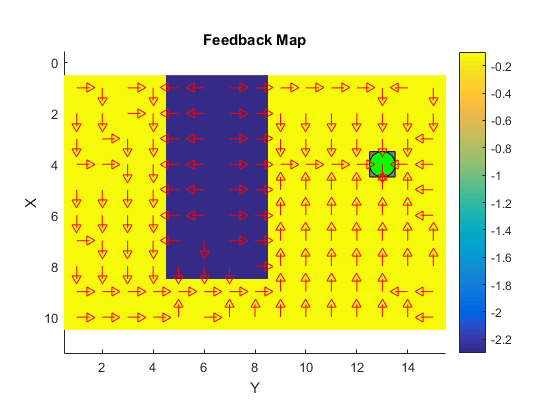
\includegraphics[width=\textwidth]{figures/1_v_low_exploration.png}
  \caption{V-function for a low exploration of $0.1$ and number of episodes set to 1000}\label{fig:1_v_low_exploration}
  \end{minipage}
    \begin{minipage}[]{0.8\textwidth}
   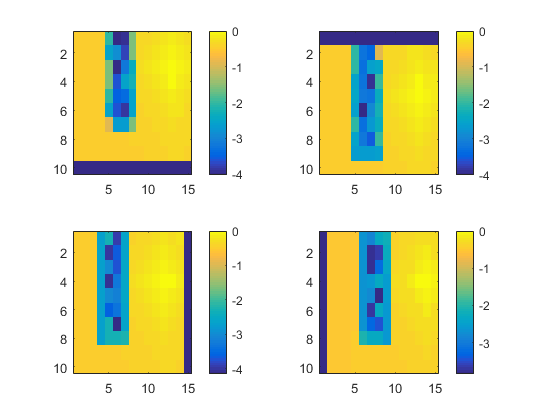
\includegraphics[width=\textwidth]{figures/1_q_low_exploration.png}
   \caption{Q-function for a low exploration of $0.1$ and number of episodes set to 1000}\label{fig:1_q_low_exploration}
  \end{minipage}
\end{figure}
\begin{table}[H]
\centering
\caption{Parameters}
\label{my-label}
\begin{tabular}{llll}
\hline
Learning rate & Discount factor & Exploration & Episodes \\ \hline
0.4 &\vline 0.9 &\vline 0.1 &\vline 1000 \\ \hline
\end{tabular}
\end{table}

\begin{figure}[H]
\centering
  \begin{minipage}[]{0.8\textwidth}
  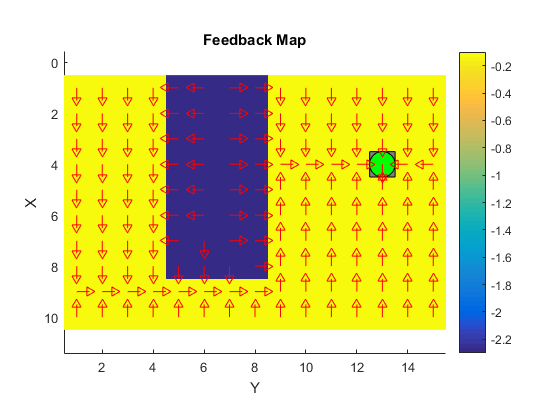
\includegraphics[width=\textwidth]{figures/1_v_high_exploration.png}
  \caption{V-function for a high exploration of $0.8$ and number of episodes set to 1000}\label{fig:1_v_high_exploration}
  \end{minipage}
    \begin{minipage}[]{0.8\textwidth}
   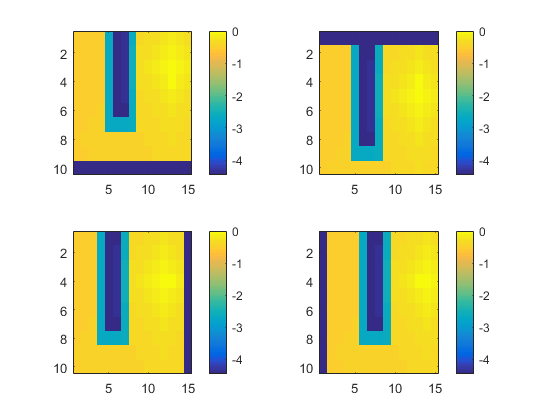
\includegraphics[width=\textwidth]{figures/1_q_high_exploration.png}
   \caption{Q-function for a high exploration of $0.8$ and number of episodes set to 1000}\label{fig:1_q_high_exploration}
  \end{minipage}
\end{figure}
\begin{table}[H]
\centering
\caption{Parameters}
\label{my-label}
\begin{tabular}{llll}
\hline
Learning rate & Discount factor & Exploration & Episodes \\ \hline
0.4 &\vline 0.9 &\vline 0.8 &\vline 1000 \\ \hline
\end{tabular}
\end{table}

As we can observe in the four figures above, it doesn't significantly matter if we start with random values in our q-function or everything set to zero. We will converge sooner or later. What we can observe is that when we set the exploration value to a low value we don't get as good convergence as with a high exploration. This could have its explanation in that once we find a way that is fairly efficient, we stick with it and doesn't walk out into the blue area to find possibly better paths to traverse.

\subsection{Sudden irritating blob}

\begin{figure}[H]
\centering
  \begin{minipage}[]{0.6\textwidth}
  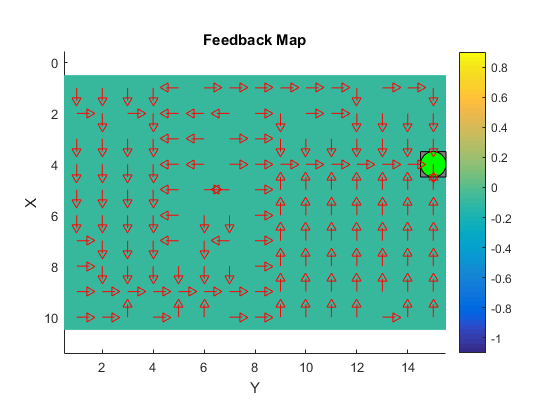
\includegraphics[width=\textwidth]{figures/2_v_low_exploration.png}
  \caption{V-function for a low exploration of $0.1$ and number of episodes set to 1000}\label{fig:2_v_low_exploration}
  \end{minipage}
    \begin{minipage}[]{0.6\textwidth}
   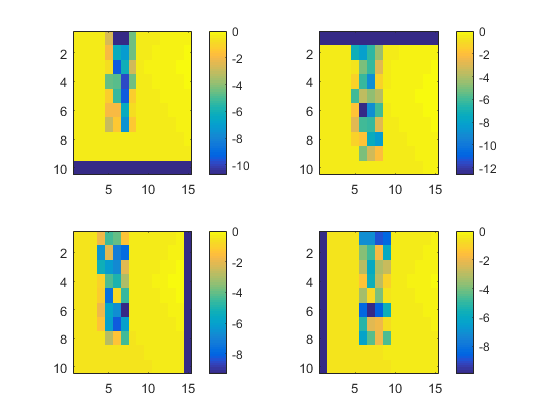
\includegraphics[width=\textwidth]{figures/2_q_low_exploration.png}
   \caption{Q-function for a low exploration of $0.1$ and number of episodes set to 1000}\label{fig:2_q_low_exploration}
  \end{minipage}
\end{figure}
\begin{table}[H]
\centering
\caption{Parameters}\label{my-label}
\begin{tabular}{llll}
\hline
Learning rate & Discount factor & Exploration & Episodes \\ \hline
0.4 &\vline 0.9 &\vline 0.1 &\vline 1000 \\ \hline
\end{tabular}
\end{table}

\begin{figure}[H]
\centering
  \begin{minipage}[]{0.6\textwidth}
  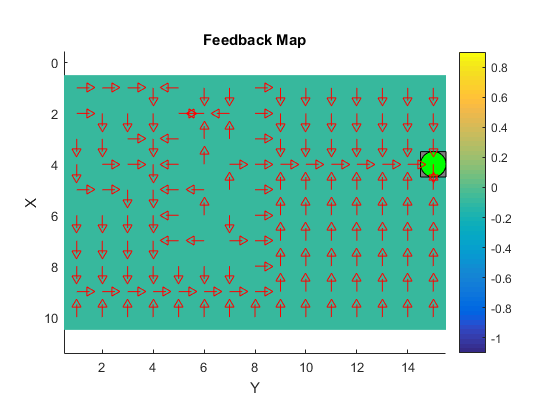
\includegraphics[width=\textwidth]{figures/2_v_high_exploration.png}
  \caption{V-function for a high exploration of $0.8$ and number of episodes set to 1000}\label{fig:2_v_high_exploration}
  \end{minipage}
    \begin{minipage}[]{0.6\textwidth}
   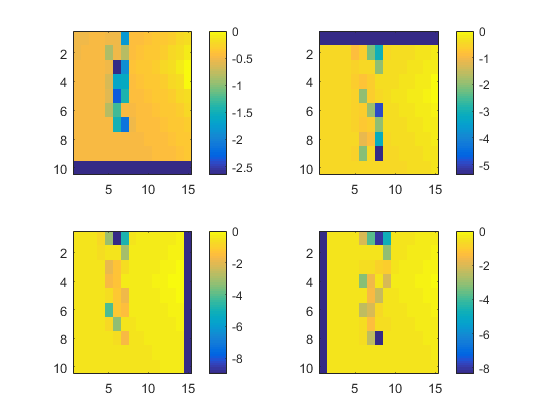
\includegraphics[width=\textwidth]{figures/2_q_high_exploration.png}
   \caption{Q-function for a high exploration of $0.8$ and number of episodes set to 1000}\label{fig:2_q_high_exploration}
  \end{minipage}
\end{figure}
\begin{table}[H]
\centering
\caption{Parameters}
\label{my-label}
\begin{tabular}{llll}
\hline
Learning rate & Discount factor & Exploration & Episodes \\ \hline
0.4 &\vline 0.9 &\vline 0.8 &\vline 1000 \\ \hline
\end{tabular}
\end{table}

Once again we can see that a low exploration results in a less explored state-space. We can also observe that we don't get as a good convergence as the first world when randomness is introduced. This could also be explained by not increasing the number of episodes before we show the result.

\begin{figure}[H]
\centering
  \begin{minipage}[]{0.6\textwidth}
  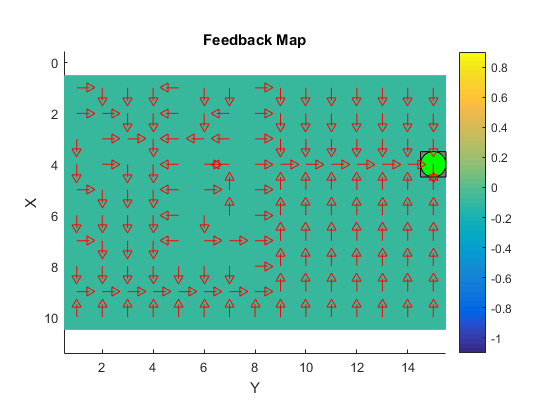
\includegraphics[width=\textwidth]{figures/2_v_high_learning.png}
  \caption{V-function for a high learning rate $0.9$ and number of episodes set to 1000}\label{fig:2_v_high_learning}
  \end{minipage}
    \begin{minipage}[]{0.6\textwidth}
   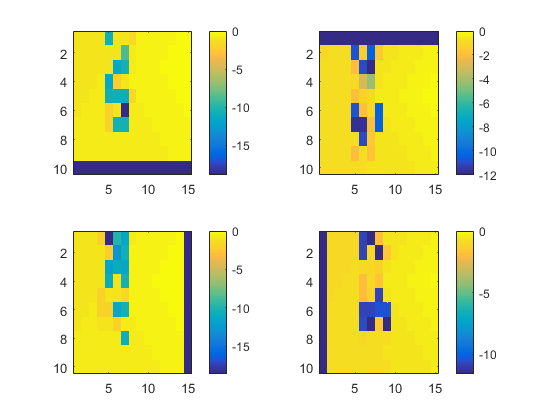
\includegraphics[width=\textwidth]{figures/2_q_high_learning.png}
   \caption{Q-function for a high learning rate $0.9$ and number of episodes set to 1000}\label{fig:2_q_high_learning}
  \end{minipage}
\end{figure}
\begin{table}[H]
\centering
\caption{Parameters}
\label{my-label}
\begin{tabular}{llll}
\hline
Learning rate & Discount factor & Exploration & Episodes \\ \hline
0.9 &\vline 0.9 &\vline 1..0 &\vline 1000 \\ \hline
\end{tabular}
\end{table}

For the two figures above we made the exploration rate dynamic but significantly increased the learning rate. We could expect that since we have some randomness in the state space, a high learning rate would be bad compared to the results above. We can observe how t V-function hasn't changed much but how the Q-function have significantly higher weights in the "random blob" area. 

Dijkstras shortest path would struggle in the "Sudden irritating blob" since we have randomness in the state space. For the static "irritating blob" Dijkstra would perform better since no randomness is present in the state space. The problem with Dijkstras shortest path  is that it consider the full path from current position to the goal instead of only looking for the expected feedback one step at a time.

\subsection{The way to HG}

In this world we have two irritating blobs with a small walk-way between and a long way around. The task is to get from one side of the blobs to the terminal state. We could expect greedy algorithms that doesn't take exploration into account to go for the small walk-way and never find a path around the blobs. 

\begin{figure}[H]
\centering
  \begin{minipage}[]{0.6\textwidth}
  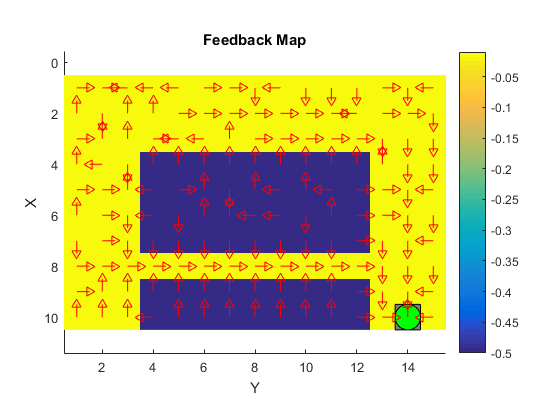
\includegraphics[width=\textwidth]{figures/3_v_low_exploration.png}
  \caption{V-function for a low exploration of $0.1$ and number of episodes set to 1000}\label{fig:3_v_low_exploration}
  \end{minipage}
    \begin{minipage}[]{0.6\textwidth}
   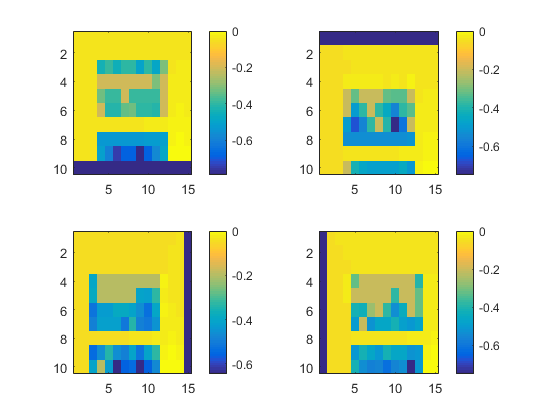
\includegraphics[width=\textwidth]{figures/3_q_low_exploration.png}
   \caption{Q-function for a low exploration of $0.1$ and number of episodes set to 1000}\label{fig:3_q_low_exploration}
  \end{minipage}
\end{figure}
\begin{table}[H]
\centering
\caption{Parameters}
\label{my-label}
\begin{tabular}{llll}
\hline
Learning rate & Discount factor & Exploration & Episodes \\ \hline
0.4 &\vline 0.9 &\vline 0.1 &\vline 1000 \\ \hline
\end{tabular}
\end{table}

\begin{figure}[H]
\centering
  \begin{minipage}[]{0.6\textwidth}
  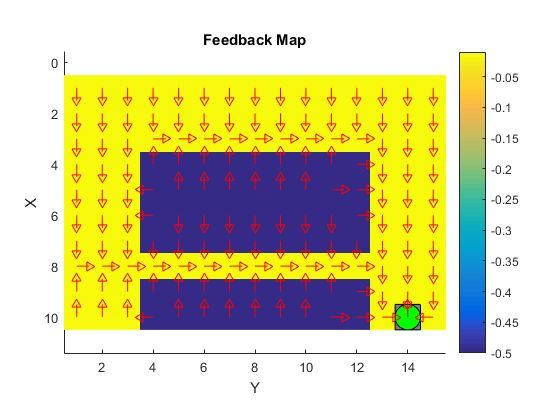
\includegraphics[width=\textwidth]{figures/3_v_high_exploration.png}
  \caption{V-function for a high exploration of $0.8$ and number of episodes set to 1000}\label{fig:3_v_high_exploration}
  \end{minipage}
    \begin{minipage}[]{0.6\textwidth}
   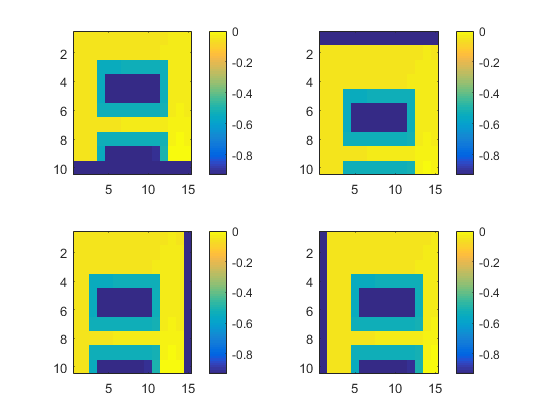
\includegraphics[width=\textwidth]{figures/3_q_high_exploration.png}
   \caption{Q-function for a high exploration of $0.8$ and number of episodes set to 1000}\label{fig:3_q_high_exploration}
  \end{minipage}
\end{figure}
\begin{table}[H]
\centering
\caption{Parameters}
\label{my-label}
\begin{tabular}{llll}
\hline
Learning rate & Discount factor & Exploration & Episodes \\ \hline
0.4 &\vline 0.9 &\vline 0.8 &\vline 1000 \\ \hline
\end{tabular}
\end{table}

In the case of "The road to HG”" we have a short path with "irritating blobs" on both sides meaning we either try to thread the needle on the short path, or walk around one of the blobs. For low exploration we see that we don't get a perfect convergence for the full state-space, while high exploration results in a full convergence to the optimal policy. This could be explained by the low exploration evaluation never consider anything other than the short-cut.

\subsection{The way back from HG}

In this world we have the same layout as the previous one but we start at HG and try to get back home. In contrast to all other worlds, this one introduce a probability of the action we take not being the action the agent performs. 

\begin{figure}[H]
\centering
  \begin{minipage}[]{0.8\textwidth}
  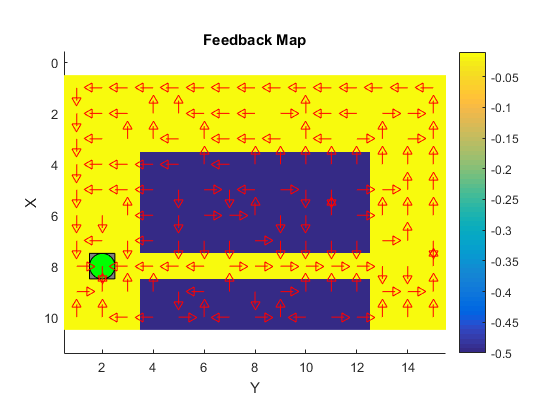
\includegraphics[width=\textwidth]{figures/4_v_low_exploration.png}
  \caption{V-function for a low exploration of $0.1$ and number of episodes set to 1000}\label{fig:4_v_low_exploration}
  \end{minipage}
    \begin{minipage}[]{0.8\textwidth}
   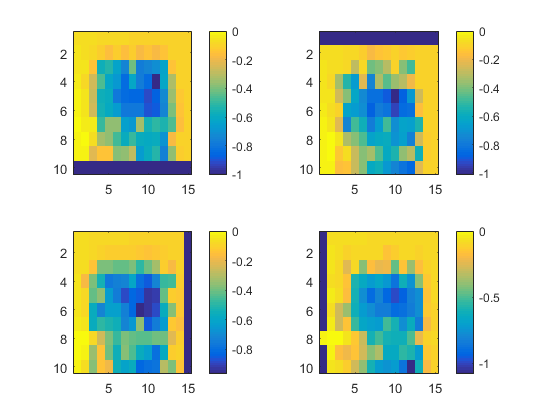
\includegraphics[width=\textwidth]{figures/4_q_low_exploration.png}
   \caption{Q-function for a low exploration of $0.1$ and number of episodes set to 1000}\label{fig:4_q_low_exploration}
  \end{minipage}
\end{figure}
\begin{table}[H]
\centering
\caption{Parameters}
\label{my-label}
\begin{tabular}{llll}
\hline
Learning rate & Discount factor & Exploration & Episodes \\ \hline
0.3 &\vline 0.9 &\vline 0.1 &\vline 1000 \\ \hline
\end{tabular}
\end{table}

\begin{figure}[H]
\centering
  \begin{minipage}[]{0.6\textwidth}
  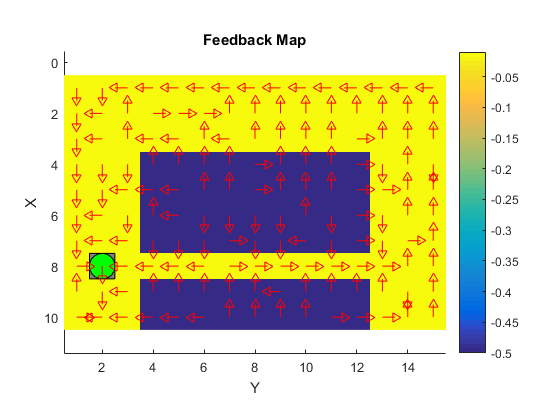
\includegraphics[width=\textwidth]{figures/4_v_high_exploration.png}
  \caption{V-function for a high exploration of $0.8$ and number of episodes set to 1000}\label{fig:4_v_high_exploration}
  \end{minipage}
    \begin{minipage}[]{0.6\textwidth}
   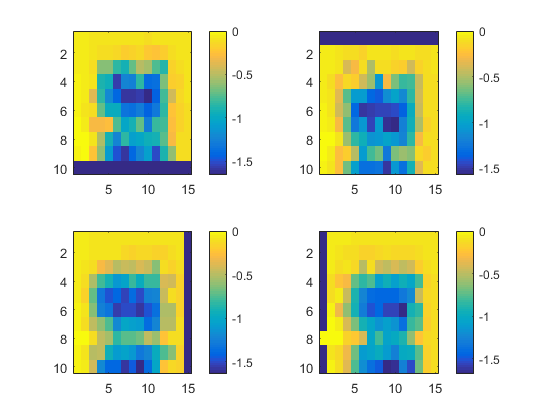
\includegraphics[width=\textwidth]{figures/4_q_high_exploration.png}
   \caption{Q-function for a high exploration of $0.8$ and number of episodes set to 1000}\label{fig:4_q_high_exploration}
  \end{minipage}
\end{figure}
\begin{table}[H]
\centering
\caption{Parameters}
\label{my-label}
\begin{tabular}{llll}
\hline
Learning rate & Discount factor & Exploration & Episodes \\ \hline
0.3 &\vline 0.9 &\vline 0.8 &\vline 1000 \\ \hline
\end{tabular}
\end{table}

We can observe from the figures above how, when we introduce a certain level of randomness in our actions, the agent with high exploration tries to get as far away from the short-cut as possible. This is caused by the probability of the agent taking a miss-step into the bad area when taking the short-cut is fairly high (p = 0.3). With low exploration we can see the same trend. We can see how we never reach full convergence. This is most likely a result of the induced random actions. With orders of magnitude higher number of episodes the random actions and rewards might converge. The most interesting observation from this world is that the Q-learning algorithm is able to find good policies even when our actions and the world-state isn't completely deterministic. 

\subsection{Conclusion}

In conclusion we have observed how, for the given worlds, the exploration factor does affect the number of episodes required for complete converge of the state space, with a low exploration we don't get convergence for the Q-function as fast compared to a high level of exploration. Neither the discount factor or the learning rate did affect the results. This could be explained by the state spaces being small and not very complex.

Since reinforcement-learning doesn't require training data or previous knowledge of the domain it will be used in it can be useful in cases where we can measure how well an agent performed but not necessarily say how it should make things differently. A variant of Q-learning called \textit{deep reinforcement learning} has seen some success in learning how to play games such as breakout and go. 

\end{document}
